% ============================================================================
% Presentation Slides — OptimShortestPaths
% Tianchi Chen & Shihua Yu
% ============================================================================
\documentclass[aspectratio=169,11pt]{beamer}

\usetheme{Madrid}
\usecolortheme{seahorse}
\setbeamertemplate{navigation symbols}{}
\setbeamertemplate{footline}[frame number]

\usepackage[utf8]{inputenc}
\usepackage[T1]{fontenc}
\usepackage{amsmath,amssymb}
\usepackage{booktabs}
\usepackage{graphicx}
\usepackage{xcolor}
\usepackage{tikz}
\usetikzlibrary{arrows.meta,positioning,shapes.geometric,calc,fit}

\newcommand{\BigO}[1]{\mathcal{O}(#1)}

\definecolor{pillblue}{HTML}{3B82F6}
\definecolor{pillgreen}{HTML}{10B981}
\definecolor{pillred}{HTML}{EF4444}
\definecolor{pillorange}{HTML}{F59E0B}
\definecolor{bglight}{HTML}{F8FAFC}

\title{Interpretable Multi-Objective Drug Repurposing\\via Shortest-Path Casting on Knowledge Graphs}
\author{Tianchi Chen \and Shihua Yu}
\institute{
\texttt{github.com/youseihuayu-wonderful/OptimShortestPaths.jl}
}
\date{}

\begin{document}

% ============================================================================
% TITLE
% ============================================================================
\begin{frame}
\titlepage
\end{frame}

% ============================================================================
% OUTLINE
% ============================================================================
\begin{frame}{Outline}
\tableofcontents
\end{frame}

% ============================================================================
\section{Research Question}
% ============================================================================

\begin{frame}{The Research Question}

\begin{block}{Central Question}
\Large Can we repurpose existing drugs for new diseases using
\textbf{interpretable graph algorithms} instead of black-box AI,
while simultaneously optimizing for \textbf{both efficacy and safety}?
\end{block}

\vspace{1em}

\textbf{Three sub-questions:}

\begin{enumerate}
    \item Can shortest-path distances on biomedical knowledge graphs
          predict drug--disease therapeutic associations?
    \item Can we add a safety dimension \emph{without} destroying
          predictive accuracy?
    \item Can recent algorithmic breakthroughs (STOC 2025) make this
          computationally practical at biomedical scale?
\end{enumerate}

\end{frame}

% ============================================================================
\section{Motivation}
% ============================================================================

\begin{frame}{Why Drug Repurposing?}

\begin{columns}[T]
\begin{column}{0.48\textwidth}
\textbf{De novo drug discovery:}
\begin{itemize}
    \item 12--15 years development
    \item \$2.6 billion average cost
    \item $>$90\% failure rate in trials
\end{itemize}

\vspace{1em}

\textbf{Drug repurposing:}
\begin{itemize}
    \item 3--5 years (known safety)
    \item $<$\$300 million
    \item Higher success rate
\end{itemize}
\end{column}

\begin{column}{0.48\textwidth}
\textbf{Real-world successes:}
\begin{itemize}
    \item Thalidomide $\to$ multiple myeloma
    \item Sildenafil $\to$ pulmonary hypertension
    \item Minoxidil $\to$ hair loss
\end{itemize}

\vspace{1em}

\textbf{Scale of opportunity:}
\begin{itemize}
    \item $\sim$4,000 approved drugs
    \item $\sim$10,000 known diseases
    \item 40 million potential pairs to screen
\end{itemize}
\end{column}
\end{columns}

\end{frame}

% ----------------------------------------------------------------------------

\begin{frame}{The Problem with Current AI Approaches}

\begin{columns}[T]
\begin{column}{0.55\textwidth}

\textbf{Knowledge Graph Embeddings (TransE, ComplEx, RotatE):}

\begin{itemize}
    \item[\textcolor{pillgreen}{\checkmark}] High accuracy (AUROC 0.85--0.92)
    \item[\textcolor{pillred}{\bfseries $\times$}] \textbf{Opaque}: produces a score, no explanation
    \item[\textcolor{pillred}{\bfseries $\times$}] \textbf{Single-objective}: conflates efficacy \& safety
    \item[\textcolor{pillred}{\bfseries $\times$}] \textbf{Not auditable}: clinicians can't verify why
\end{itemize}

\vspace{1em}

\textbf{What clinicians actually need:}
\begin{itemize}
    \item \emph{``Why is this drug predicted to work?''}
    \item \emph{``What are the safety trade-offs?''}
    \item \emph{``What biological mechanism mediates this?''}
\end{itemize}

\end{column}

\begin{column}{0.42\textwidth}
\centering

\textbf{Black-box output:}

\medskip

\begin{tabular}{lc}
\toprule
Drug & Score \\
\midrule
Drug A & 0.87 \\
Drug B & 0.82 \\
Drug C & 0.79 \\
\bottomrule
\end{tabular}

\vspace{0.5em}
{\small \textcolor{pillred}{$\to$ Why? No idea.}}

\vspace{1.5em}

\textbf{Our output:}

\medskip

{\small Drug A $\xrightarrow{\text{binds}}$ Gene X $\xrightarrow{\text{assoc.}}$ Disease}

\vspace{0.5em}
{\small \textcolor{pillgreen}{$\to$ Testable biological hypothesis}}

\end{column}
\end{columns}

\end{frame}

% ============================================================================
\section{Core Philosophy}
% ============================================================================

\begin{frame}{Core Philosophy: Problem Casting}

\begin{block}{Key Insight}
Don't learn latent representations --- \textbf{transform the problem}
into one with known optimal solutions.
\end{block}

\vspace{0.6em}

\begin{center}
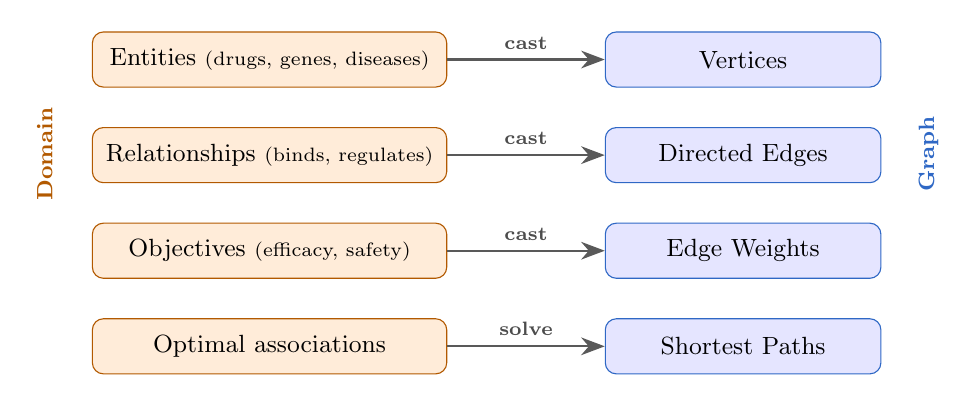
\begin{tikzpicture}[
    dombox/.style={rectangle, draw=orange!70!black, fill=orange!15, rounded corners=4pt,
                   minimum width=4.5cm, minimum height=0.7cm, font=\small, align=center},
    gphbox/.style={rectangle, draw=pillblue!80!black, fill=blue!10, rounded corners=4pt,
                   minimum width=3.5cm, minimum height=0.7cm, font=\small, align=center},
    arr/.style={-{Stealth[length=3mm]}, thick, gray!70!black},
    castlbl/.style={font=\scriptsize\bfseries, text=gray!60!black, above, midway},
    node distance=0.5cm
]
\node[dombox] (e) {Entities \scriptsize(drugs, genes, diseases)};
\node[gphbox, right=2cm of e] (v) {Vertices};
\node[dombox, below=of e] (r) {Relationships \scriptsize(binds, regulates)};
\node[gphbox, right=2cm of r] (ed) {Directed Edges};
\node[dombox, below=of r] (o) {Objectives \scriptsize(efficacy, safety)};
\node[gphbox, right=2cm of o] (w) {Edge Weights};
\node[dombox, below=of o] (s) {Optimal associations};
\node[gphbox, right=2cm of s] (p) {Shortest Paths};

\draw[arr] (e) -- node[castlbl] {cast} (v);
\draw[arr] (r) -- node[castlbl] {cast} (ed);
\draw[arr] (o) -- node[castlbl] {cast} (w);
\draw[arr] (s) -- node[castlbl] {solve} (p);

% Brace labels
\node[font=\footnotesize\bfseries, text=orange!70!black, rotate=90] at ($(e.west)+(-0.6,-1.2)$) {Domain};
\node[font=\footnotesize\bfseries, text=pillblue!80!black, rotate=90] at ($(v.east)+(0.6,-1.2)$) {Graph};
\end{tikzpicture}
\end{center}

\vspace{0.3em}

\textbf{Result}: Interpretability is \emph{structural}, not post-hoc.
The path \emph{is} the explanation.

\end{frame}

% ----------------------------------------------------------------------------

\begin{frame}{Learn vs.\ Cast: Two Paradigms}

\begin{columns}[T]
\begin{column}{0.48\textwidth}
\textbf{Embedding approach (learn):}
\begin{itemize}
    \item Train model on graph
    \item Get opaque score
    \item Apply SHAP/LIME \emph{after} to ``explain''
    \item Explanation $\neq$ mechanism
\end{itemize}

\vspace{0.5em}
\textcolor{pillred}{Post-hoc explanations can be misleading}
\end{column}

\begin{column}{0.48\textwidth}
\textbf{Our approach (cast):}
\begin{itemize}
    \item Transform problem to shortest paths
    \item Solve optimally (exact algorithm)
    \item Path = prediction = explanation
    \item Every intermediate node is verifiable
\end{itemize}

\vspace{0.5em}
\textcolor{pillgreen}{Explanation is the computation itself}
\end{column}
\end{columns}

\vspace{1.2em}

\begin{block}{Design Principle}
\centering
\textbf{Interpretability should be a property of the method,\\
not an afterthought applied to an opaque model.}
\end{block}

\end{frame}

% ============================================================================
\section{Data: Hetionet Knowledge Graph}
% ============================================================================

\begin{frame}{Data: Hetionet v1.0 Knowledge Graph}

\begin{columns}[T]
\begin{column}{0.5\textwidth}

\begin{center}
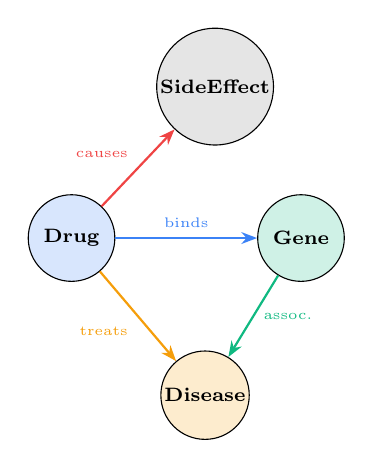
\begin{tikzpicture}[
    ntype/.style={circle, draw, minimum size=1.1cm, font=\scriptsize\bfseries, inner sep=1pt},
    edge/.style={-{Stealth[length=2mm]}, thick},
    node distance=1.8cm
]
\node[ntype, fill=pillblue!20] (comp) {Drug};
\node[ntype, fill=pillgreen!20, right=of comp] (gene) {Gene};
\node[ntype, fill=pillorange!20, below right=1.2cm and 0.9cm of comp] (dis) {Disease};
\node[ntype, fill=gray!20, above right=1cm and 0.9cm of comp] (se) {Side\\Effect};

\draw[edge, pillblue] (comp) -- node[above, font=\tiny] {binds} (gene);
\draw[edge, pillgreen] (gene) -- node[right, font=\tiny] {assoc.} (dis);
\draw[edge, pillorange] (comp) -- node[below left, font=\tiny] {treats} (dis);
\draw[edge, pillred] (comp) -- node[above left, font=\tiny] {causes} (se);
\end{tikzpicture}
\end{center}

\vspace{0.5em}

\textbf{Key edge types used:}
\begin{itemize}
    \item \textcolor{pillblue}{Compound--binds--Gene}
    \item \textcolor{pillgreen}{Gene--associates--Disease}
    \item \textcolor{pillorange}{Compound--treats--Disease}
    \item \textcolor{pillred}{Compound--causes--Side Effect}
\end{itemize}

\end{column}

\begin{column}{0.47\textwidth}

\begin{table}
\centering
\begin{tabular}{lr}
\toprule
\textbf{Statistic} & \textbf{Value} \\
\midrule
Node types & 11 \\
Edge types & 24 \\
Total nodes & 47,031 \\
Total edges & 2,250,197 \\
\midrule
Compounds & 1,552 \\
Diseases & 137 \\
Genes & 20,945 \\
Side effects & 5,734 \\
\midrule
\multicolumn{2}{l}{\textbf{Evaluation}} \\
PharmacotherapyDB & 755 \\
\quad indications & \\
Evaluation pairs & 53,019 \\
\bottomrule
\end{tabular}
\end{table}

\end{column}
\end{columns}

\end{frame}

% ============================================================================
\section{Proposed Solution}
% ============================================================================

\begin{frame}{End-to-End Pipeline}

\begin{center}
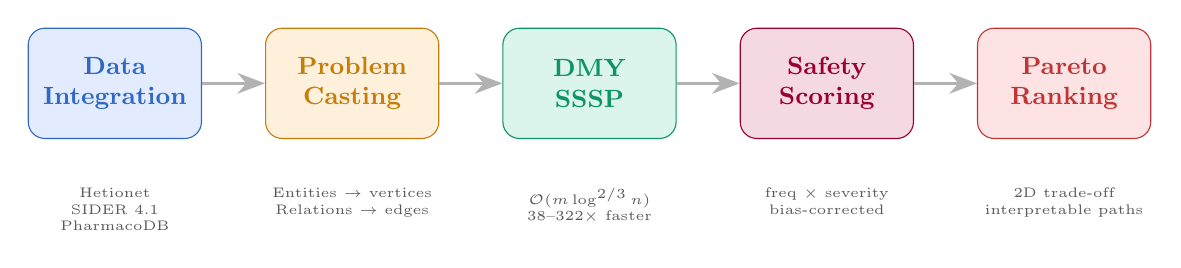
\begin{tikzpicture}[
    stage/.style={rectangle, draw=#1!80!black, fill=#1!15, rounded corners=6pt,
                  minimum width=2.2cm, minimum height=1.4cm, font=\small\bfseries,
                  align=center, text=#1!80!black},
    arr/.style={-{Stealth[length=3.5mm]}, very thick, gray!60},
    note/.style={font=\tiny, text=gray!70!black, align=center}
]
\node[stage=pillblue] (data) {Data\\Integration};
\node[stage=pillorange, right=0.8cm of data] (cast) {Problem\\Casting};
\node[stage=pillgreen, right=0.8cm of cast] (dmy) {DMY\\SSSP};
\node[stage=purple, right=0.8cm of dmy] (safe) {Safety\\Scoring};
\node[stage=pillred, right=0.8cm of safe] (pareto) {Pareto\\Ranking};

\draw[arr] (data) -- (cast);
\draw[arr] (cast) -- (dmy);
\draw[arr] (dmy) -- (safe);
\draw[arr] (safe) -- (pareto);

\node[note, below=0.5cm of data] {Hetionet\\SIDER 4.1\\PharmacoDB};
\node[note, below=0.5cm of cast] {Entities $\to$ vertices\\Relations $\to$ edges};
\node[note, below=0.5cm of dmy] {$\BigO{m\log^{2/3}n}$\\38--322$\times$ faster};
\node[note, below=0.5cm of safe] {freq $\times$ severity\\bias-corrected};
\node[note, below=0.5cm of pareto] {2D trade-off\\interpretable paths};
\end{tikzpicture}
\end{center}

\vspace{1em}

\textbf{Key property}: Every stage is transparent.
\begin{itemize}
    \item \textbf{Input}: public, curated knowledge graphs (no proprietary data)
    \item \textbf{Algorithm}: exact optimal solution (not approximate or learned)
    \item \textbf{Output}: ranked drugs with traceable biological paths + safety profiles
\end{itemize}

\end{frame}

% ----------------------------------------------------------------------------

\begin{frame}{Pillar 1: The DMY Algorithm (STOC 2025)}

\textbf{Classical barrier:} Dijkstra's algorithm is $\BigO{(m+n) \log n}$ --- optimal since 1959.

\vspace{0.3em}

\textbf{Breakthrough (Duan, Mao \& Yin, STOC 2025):}
$\BigO{m \log^{2/3} n}$ via recursive frontier sparsification.

\vspace{0.8em}

\begin{table}
\centering
\begin{tabular}{lrrrr}
\toprule
\textbf{Graph} & \textbf{$|V|$} & \textbf{$|E|$} & \textbf{DMY time} & \textbf{Speedup} \\
\midrule
Hetionet (real) & 47,031 & 450,000 & 103 ms & \textbf{38.5$\times$} \\
Synthetic & 100,000 & 1,000,000 & 338 ms & \textbf{149.9$\times$} \\
Synthetic & 500,000 & 5,000,000 & 1.6 s & \textbf{321.9$\times$} \\
\bottomrule
\end{tabular}
\end{table}

\vspace{0.5em}

\begin{columns}[T]
\begin{column}{0.48\textwidth}
\textbf{Correctness:}\\
47,031/47,031 distances match Dijkstra\\
(zero numerical discrepancy)
\end{column}
\begin{column}{0.48\textwidth}
\textbf{Practical impact:}\\
1,552 drugs $\times$ 137 diseases:\\
\textbf{42\,s} vs.\ 28\,min (Dijkstra)
\end{column}
\end{columns}

\end{frame}

% ----------------------------------------------------------------------------

\begin{frame}{Pillar 2: Multi-Objective Pareto Ranking}

\begin{columns}[T]
\begin{column}{0.55\textwidth}

\textbf{Single-objective problem:}\\
Rank by efficacy alone $\to$ ignore toxicity.

\vspace{0.8em}

\textbf{Our approach:}\\
Each drug--disease pair mapped to 2D:
\[
\mathbf{v} = (\underbrace{d_{\text{eff}}}_{\text{efficacy cost}},\ \underbrace{S(c)}_{\text{safety cost}})
\]

\textbf{Pareto front}: set of drugs where you\\
can't improve one without worsening the other.

\vspace{0.8em}

\textbf{Knee point} (via marginal rate of substitution)\\
identifies the best-balanced candidate.

\vspace{0.5em}

\textbf{Result}: 4 clinically validated treatments\\
recovered that single-objective ranking misses.

\end{column}

\begin{column}{0.42\textwidth}

\begin{center}
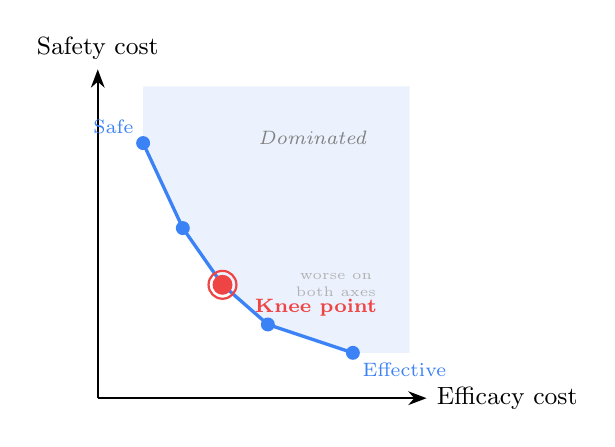
\begin{tikzpicture}[scale=0.72]
\draw[-{Stealth}, thick] (0,0) -- (5.8,0) node[right, font=\small] {Efficacy cost};
\draw[-{Stealth}, thick] (0,0) -- (0,5.8) node[above, font=\small] {Safety cost};

% Dominated points
\fill[gray!40] (2.5,3.5) circle (2.5pt);
\fill[gray!40] (3.5,3.0) circle (2.5pt);
\fill[gray!40] (4.0,2.5) circle (2.5pt);
\fill[gray!40] (3.0,4.0) circle (2.5pt);
\fill[gray!40] (4.5,3.5) circle (2.5pt);
\fill[gray!40] (1.8,4.8) circle (2.5pt);
\fill[gray!40] (3.8,4.2) circle (2.5pt);

% Pareto front (shaded region)
\fill[pillblue!10] (0.8,5.5) -- (0.8,4.5) -- (1.5,3.0) -- (2.2,2.0) -- (3.0,1.3) -- (4.5,0.8) -- (5.5,0.8) -- (5.5,5.5) -- cycle;

% Pareto front line
\draw[pillblue, very thick]
    (0.8,4.5) -- (1.5,3.0) -- (2.2,2.0) -- (3.0,1.3) -- (4.5,0.8);

% Non-dominated points
\fill[pillblue] (0.8,4.5) circle (3.5pt);
\fill[pillblue] (1.5,3.0) circle (3.5pt);
\fill[pillblue] (3.0,1.3) circle (3.5pt);
\fill[pillblue] (4.5,0.8) circle (3.5pt);

% Knee point (highlighted)
\fill[pillred] (2.2,2.0) circle (5pt);
\draw[pillred, thick] (2.2,2.0) circle (7pt);
\node[pillred, font=\scriptsize\bfseries, right] at (2.6,1.6) {Knee point};

% Labels
\node[font=\scriptsize, pillblue, above left] at (0.8,4.5) {Safe};
\node[font=\scriptsize, pillblue, below right] at (4.5,0.8) {Effective};
\node[font=\scriptsize, gray] at (3.8,4.6) {\textit{Dominated}};

% Dominated region label
\node[font=\tiny, gray!60, align=center] at (4.2,2.0) {worse on\\both axes};
\end{tikzpicture}
\end{center}

\end{column}
\end{columns}

\end{frame}

% ----------------------------------------------------------------------------

\begin{frame}{Pillar 3: Bias-Corrected Safety Scoring}

\textbf{Problem}: Raw side-effect counts are \textbf{anti-predictive}.

\vspace{0.3em}

{\small Well-studied effective drugs have \emph{more} documented adverse events
(Weber effect) $\to$ raw count \emph{penalizes} good drugs.}

\vspace{0.8em}

\textbf{Our solution} (SIDER 4.1 + CTCAE v5.0):

\[
\boxed{
S(c) = \frac{\displaystyle\sum_{t \in \text{PT}(c)} f_t \cdot g(\text{severity}_t)}
{\log(1 + |\text{PT}(c)|)}
}
\]

\vspace{0.3em}

\begin{columns}[T]
\begin{column}{0.55\textwidth}
\begin{itemize}
    \item $f_t$: label frequency from FDA package inserts\\
          {\scriptsize (not FAERS spontaneous reports)}
    \item $g(\cdot)$: CTCAE v5.0 severity grade\\
          {\scriptsize 5=fatal, 4=life-threatening, \ldots, 1=mild}
    \item Denominator: log-normalization\\
          {\scriptsize controls for label depth / reporting bias}
\end{itemize}
\end{column}
\begin{column}{0.42\textwidth}
\begin{itemize}
    \item 515 compounds with SIDER data
    \item 1,037 compounds use fallback\\
          {\scriptsize (Hetionet \emph{causes} edge counts,\\log-normalized, scaled to p75)}
    \item 12/12 validation tests pass
\end{itemize}
\end{column}
\end{columns}

\end{frame}

% ----------------------------------------------------------------------------

\begin{frame}{Safety Scoring: AUROC Impact}

\begin{center}
\begin{table}
\centering
\large
\begin{tabular}{lccl}
\toprule
\textbf{Safety method} & \textbf{AUROC} & $\Delta$ \textbf{vs.\ 1D} & \\
\midrule
No safety (1D baseline) & 0.7717 & --- & \\
Raw side-effect count & 0.6385 & \textcolor{pillred}{$-$0.133} & \textcolor{pillred}{$\blacktriangledown$ Anti-predictive} \\
SIDER freq $\times$ severity & 0.7047 & \textcolor{pillorange}{$-$0.067} & \textcolor{pillorange}{$\blacktriangledown$ Halved damage} \\
SIDER + fallback & 0.7188 & \textcolor{pillgreen!80!black}{$-$0.053} & \textcolor{pillgreen!80!black}{$\blacktriangledown$ Best 2D} \\
\bottomrule
\end{tabular}
\end{table}
\end{center}

\vspace{1em}

\begin{block}{Key finding}
\centering
Bias correction \textbf{cuts AUROC damage by 60\%} (0.133 $\to$ 0.053),\\[4pt]
making multi-objective ranking \textbf{viable} for the first time on this benchmark.
\end{block}

\vspace{0.5em}

{\small Note: Some AUROC cost is \emph{fundamental} --- adding safety \emph{necessarily}
reranks some true positives. A 2D metric that rewards avoiding toxic predictions
would show this more favorably.}

\end{frame}

% ============================================================================
\section{Results}
% ============================================================================

\begin{frame}{Case Studies: Pareto-Rescued Drugs}

\begin{table}
\centering
\large
\begin{tabular}{llcccc}
\toprule
\textbf{Drug} & \textbf{Disease} & \textbf{1D rank} & \textbf{Pareto rank} & $\Delta$ & \textbf{Validated?} \\
\midrule
Cytarabine & Leukemia & 24 & \textbf{6} & +18 & \textcolor{pillgreen}{\checkmark} \\
Moexipril & Hypertension & 12 & \textbf{5} & +7 & \textcolor{pillgreen}{\checkmark} \\
Chlorambucil & Breast cancer & 111 & \textbf{6} & +105 & \textcolor{pillgreen}{\checkmark} \\
\bottomrule
\end{tabular}
\end{table}

\vspace{0.8em}

\textbf{Example}: Chlorambucil for breast cancer

\begin{center}
\large
Chlorambucil $\xrightarrow{\text{binds}}$ \textbf{GSTP1} $\xrightarrow{\text{associates}}$ Breast Cancer
\end{center}

\vspace{0.5em}

\begin{itemize}
    \item GSTP1 (Glutathione S-transferase Pi 1) --- known mediator of alkylating
          agent resistance in breast cancer
    \item Ranked 111th by efficacy alone --- \textbf{invisible} in a top-50 screen
    \item Pareto analysis promotes it to rank 6: favorable safety + moderate efficacy
    \item The path \emph{is} the hypothesis --- directly testable by domain experts
\end{itemize}

\end{frame}

% ============================================================================
\section{Critical Comments \& Insights}
% ============================================================================

\begin{frame}{What Works Well}

\vspace{0.5em}

\renewcommand{\arraystretch}{1.6}
\begin{tabular}{cl}
\textcolor{pillgreen}{\Large\checkmark} &
\begin{minipage}[t]{0.85\textwidth}
\textbf{Interpretability is structural, not cosmetic}\\[-2pt]
{\small Every prediction = traceable biological path. Clinicians can verify each intermediate node.}
\end{minipage} \\

\textcolor{pillgreen}{\Large\checkmark} &
\begin{minipage}[t]{0.85\textwidth}
\textbf{38--322$\times$ speedup, exact correctness}\\[-2pt]
{\small First biomedical application of STOC 2025 DMY algorithm. 100\% distance match vs.\ Dijkstra.}
\end{minipage} \\

\textcolor{pillgreen}{\Large\checkmark} &
\begin{minipage}[t]{0.85\textwidth}
\textbf{Pareto ranking recovers validated treatments}\\[-2pt]
{\small 4 clinically used drugs recovered in top-50 that 1D ranking misses entirely.}
\end{minipage} \\

\textcolor{pillgreen}{\Large\checkmark} &
\begin{minipage}[t]{0.85\textwidth}
\textbf{Safety bias correction halves AUROC damage}\\[-2pt]
{\small Weber effect successfully mitigated: $-$0.133 $\to$ $-$0.053.}
\end{minipage} \\
\end{tabular}

\end{frame}

% ----------------------------------------------------------------------------

\begin{frame}{Honest Limitations}

\vspace{0.5em}

\renewcommand{\arraystretch}{1.6}
\begin{tabular}{cl}
\textcolor{pillorange}{\Large !} &
\begin{minipage}[t]{0.85\textwidth}
\textbf{AUROC gap: 0.77 vs.\ 0.85--0.92 (KGE methods)}\\[-2pt]
{\small Different tasks (link prediction vs.\ therapeutic association), but the gap is real.\\
We trade accuracy for interpretability --- a deliberate design choice.}
\end{minipage} \\

\textcolor{pillorange}{\Large !} &
\begin{minipage}[t]{0.85\textwidth}
\textbf{Binary graph limits discrimination}\\[-2pt]
{\small Hetionet edges are 0/1. Same edge-type pattern $\to$ identical scores.\\
Continuous weights (ChEMBL IC$_{50}$) would be the highest-impact upgrade.}
\end{minipage} \\

\textcolor{pillorange}{\Large !} &
\begin{minipage}[t]{0.85\textwidth}
\textbf{SIDER coverage: 33.2\% (515/1,552)}\\[-2pt]
{\small Two-thirds of compounds rely on fallback scoring.\\
Richer safety databases would substantially improve the safety dimension.}
\end{minipage} \\

\textcolor{pillorange}{\Large !} &
\begin{minipage}[t]{0.85\textwidth}
\textbf{Safety necessarily costs AUROC on 1D benchmarks}\\[-2pt]
{\small This is a fundamental trade-off, not a bug. Need 2D evaluation metrics.}
\end{minipage} \\
\end{tabular}

\end{frame}

% ----------------------------------------------------------------------------

\begin{frame}{Complementarity, Not Competition}

\begin{center}
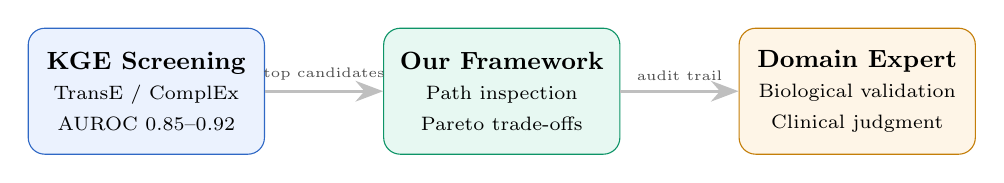
\begin{tikzpicture}[
    box/.style={rectangle, draw=#1!80!black, fill=#1!10, rounded corners=6pt,
                minimum width=3cm, minimum height=1.6cm, font=\small, align=center},
    arr/.style={-{Stealth[length=3.5mm]}, very thick, gray!50},
    note/.style={font=\tiny, text=gray!60!black, align=center, above}
]
\node[box=pillblue] (kge) {\textbf{KGE Screening}\\{\scriptsize TransE / ComplEx}\\{\scriptsize AUROC 0.85--0.92}};
\node[box=pillgreen, right=1.5cm of kge] (ours) {\textbf{Our Framework}\\{\scriptsize Path inspection}\\{\scriptsize Pareto trade-offs}};
\node[box=pillorange, right=1.5cm of ours] (expert) {\textbf{Domain Expert}\\{\scriptsize Biological validation}\\{\scriptsize Clinical judgment}};

\draw[arr] (kge) -- node[note] {top candidates} (ours);
\draw[arr] (ours) -- node[note] {audit trail} (expert);
\end{tikzpicture}
\end{center}

\vspace{1em}

\begin{columns}[T]
\begin{column}{0.48\textwidth}
\textbf{KGE methods provide:}
\begin{itemize}
    \item Fast initial screening
    \item High recall
    \item Scalable training
\end{itemize}
\end{column}
\begin{column}{0.48\textwidth}
\textbf{Our framework provides:}
\begin{itemize}
    \item \emph{Why} this drug? (path)
    \item \emph{How safe?} (Pareto front)
    \item \emph{What mechanism?} (intermediate nodes)
\end{itemize}
\end{column}
\end{columns}

\vspace{0.8em}

\centering
{\small \textbf{Analogy}: KGE is the fast detector; ours is the careful second opinion with documented reasoning.}

\end{frame}

% ============================================================================
\section{Future Work}
% ============================================================================

\begin{frame}{Future Work}

\textbf{Near-term (strengthens the paper):}
\begin{enumerate}
    \item \textbf{KGE baselines on same split} --- TransE/ComplEx via PyKEEN
          for direct, fair AUROC comparison
    \item \textbf{Continuous edge weights} --- ChEMBL IC$_{50}$, expression
          fold-changes to break the binary ceiling
    \item \textbf{Multi-objective evaluation metric} --- a metric that \emph{rewards}
          avoiding toxic predictions, not just maximizing recall
\end{enumerate}

\vspace{1em}

\textbf{Longer-term (strengthens the impact):}
\begin{enumerate}
    \setcounter{enumi}{3}
    \item \textbf{Prospective validation} --- literature review or expert
          panel on Pareto-rescued candidates
    \item \textbf{KGE--path hybrid} --- use embedding scores as edge weights
          in our framework (best of both worlds)
    \item \textbf{ChemPath interactive app} --- chatbot for researchers
          to explore drug repurposing hypotheses conversationally
\end{enumerate}

\end{frame}

% ============================================================================

\begin{frame}{Summary}

\begin{center}
\large

\textbf{Research Question}\\[4pt]
{\normalsize Can interpretable graph algorithms repurpose drugs\\
with explicit efficacy--safety trade-offs?}

\vspace{0.8em}

\textbf{Answer: Yes, with honest caveats.}

\vspace{0.8em}

\renewcommand{\arraystretch}{1.3}
\begin{tabular}{rl}
\textcolor{pillgreen}{\bfseries\checkmark} & 38--322$\times$ faster than Dijkstra (exact correctness) \\
\textcolor{pillgreen}{\bfseries\checkmark} & AUROC 0.77 on 755 therapeutic indications \\
\textcolor{pillgreen}{\bfseries\checkmark} & 4 Pareto-rescued validated treatments in top-50 \\
\textcolor{pillgreen}{\bfseries\checkmark} & Every prediction = interpretable biological path \\
\textcolor{pillorange}{\bfseries $\sim$} & Safety adds $-$0.053 AUROC (trade-off, not failure) \\
\textcolor{pillred}{\bfseries $\times$} & Below KGE accuracy (0.77 vs.\ 0.85--0.92) \\
\end{tabular}

\vspace{1.2em}

{\normalsize \textbf{Core insight}: Interpretability and multi-objective\\
optimization are worth a modest accuracy trade-off ---\\
especially when the alternative is an unexplainable black box.}

\end{center}

\end{frame}

% ============================================================================

\begin{frame}{}
\centering
\vspace{2em}
{\Huge Thank You}

\vspace{1.5em}

{\large Tianchi Chen \quad \& \quad Shihua Yu}

\vspace{1em}

{\normalsize
\texttt{github.com/youseihuayu-wonderful/OptimShortestPaths.jl}
}

\vspace{2em}

{\small Questions?}

\end{frame}

\end{document}
